%-------------------------------------------
% En-tête type de document pour le projet PLD
% Il suffit de remplir le input ligne 45
%-------------------------------------------

\documentclass[a4paper]{article}

\usepackage[utf8]{inputenc}   
\usepackage[top=2cm, bottom=2cm, left=2cm, right=2cm]{geometry}
\usepackage{ucs}
% Reconnaitre les caratères accentués dans le source.
\usepackage[T1]{fontenc} 
\usepackage{lmodern}
\usepackage[francais]{babel}
% Insertion d'images
\usepackage{graphicx}
% Utilisation du symbole EURO
\usepackage{eurosym}

\begin{document}

%------------------------------------- Page de titre
\begin{titlepage}
~ 
\vfill
	\begin{center}
		\begin{Huge}
		Projet d'Ingénierie : Dossier de Synthèse\\
		\end{Huge} 
\vfill
		\textbf{Hexanome 4111 :} 
		\\Quentin \bsc{Calvez}, Matthieu \bsc{Coquet}, 
		\\Jan \bsc{Keromnes}, Alexandre \bsc{Lefoulon}, 
		\\Thaddée \bsc{Tyl}, Xavier \bsc{Sauvagnat},
		\\Tuuli \bsc{Tyrväinen}
\vfill		
		\begin{Large}
		Février 2012
		\end{Large}
\vfill
	\begin{tabular}{|c|c|c|c|c|}
 	 \hline
   Destinataire & Version & Etat & Dernière révision & Equipe \\
   \hline
   Client & 1 & Validé & \today & H4111 \\
   \hline
	\end{tabular}
	\end{center}
\vfill
\end{titlepage}
%----------------------------------------------------
%--------------------------------- Table des matières
\newpage
\tableofcontents
\newpage
%----------------------------------------------------


\section{Introduction}

Ce document présente de manière synthétique la solution retenue pour répondre à l'appel d'offre de la COPEVUE: "Système de monitoring à distance de sites isolés".

Dans ce document seront présentés les différents aspects du futur système ainsi que les fonctionnalités qui lui seront associées.

\subsection{Terminologies et Abréviations}

Voir document ``glossaire-commun''.

\subsection{Cadre de l’étude et objectif}

Le COPEVUE (Comité Pour la Protection de l'EnVironnement de l'Union Européenne) souhaite étudier un système de monitoring à distance de sites isolés. L'objectif est d'étudier et de concevoir un système complet, autonome et générique de mesure et de monitoring ainsi que le pilotage, la configuration et la maintenance à distance de ces stations. Le résultat doit constituer une solution évolutive, autonome, fiable et déployable à l'échelle européenne. Ce système se veut être un parfait palliatif aux dysfonctionnements actuels en apportant une réponse aux problématiques détaillées ci-dessous.

De nombreuses régions d'Europe sont faiblement desservies pour des raisons :

démographiques, le faible peuplement de ces zones fait que les infrastructures de transport sont peu développées.
géographiques, certaines de ces zones sont difficilement accessibles par la difficulté et le coût d'installation d'infrastructures.
La problématique réside ici en la capacité d'autonomie des stations isolées (en énergie, déchets, présence humaine, etc.). Ces stations doivent être régulièrement surveillées pour veiller à un fonctionnement optimale tout en évitant les risques environnementaux. Ces visites permettent de s'assurer que les stations sont bien ravitaillées, nettoyées, vidées et fonctionnelles.

A l'échelle européenne il n'existe aucun organisme centralisé et donc aucun système de gestion chargé de la surveillance de sites distants isolés. Notre solution vise donc à informatiser ce système d'information que ce soit au niveau des sites distants ou par la mise en place d'un site central de monitoring. Il s'agit avant tout d'un projet technique mais qui pose de solides fondations quant à la mise en place d'un organisme visant à fédérer l'ensemble des acteurs européens.

Pour cet appel d'offre, seront visées uniquement les stations réservoirs utilisées pour stocker des liquides (eau, carburant et autres substances) ou bien des déchets.

\subsection{Rappel synthétique des critiques de l’existant}

La décentralisation de la surveillance des sites isolés est source de nombreux dysfonctionnements qui peuvent être déclinés en deux grandes catégories :

\begin{itemize}
\item un gaspillage financier (argent provenant pour la majorité des cas des contribuables),
\item un risque environnemental important, non contrôlé.
\end{itemize}

Plusieurs facteurs sont sources de gaspillage financier :

\begin{itemize}
\item La logistique. Il n'existe pas de planification globale et donc pas d'optimisation dans les livraisons/enlèvements de contenant et systématiquement un camion se retrouve avec un chargement nul sur un des trajets (l'aller ou le retour).
\item La surveillance. Celle-ci est effectuée par des opérationnels et est donc fortement coûteuse, en particulier lorsque l'on constate que la majorité des déplacements ne débouchent sur aucune opération de maintenance. Il s'agit donc d'une monopolisation des ressources humaines et matérielles pour une tâche sans réelle valeur ajoutée par rapport à ce qu'elle pourrait apporter.
\item Une surveillance non globale. L'éparpillement de la gestion de ces sites empêche de faire des économies d'échelles à de nombreux niveaux que ce soit au niveau de la surveillance ou bien dans la mise en commun des achats de contenant ou de services de transport.
\end{itemize}

De nombreux points favorisent les risques environnementaux :

\begin{itemize}
\item Oublis. Le système reposant uniquement sur des ressources humaines, de nombreux oublis de ravitaillement de cuves ont été constatés. C'est totalement inacceptable pour des cuves stratégiques comme celles dédiées à la lutte contre les incendies.
\item Fuites. En plus d'être une perte financière, les fuites, suivant le contenant de la cuve, peuvent s'avérer très dangereuses d'un point de vue écologique. Le problème est que ces fuites sont constatées bien souvent trop tard du fait d'une surveillance manuelle, souvent fortement espacée dans le temps.
\end{itemize}

D'une manière générale, il manque une traçabilité des opérations effectuées par les divers acteurs et ne permet donc pas un monitoring global.

\subsection{Description des axes de progrès}

Deux axes de progrès ont été retenus:

\paragraph{Gain en termes de coûts directs}

\begin{itemize}
\item Centralisation de la surveillance : économies d'échelle.
\item Une meilleure logistique, notamment en termes de transport.
\item Des ressources humaines mieux utilisées. Les opérationnels doivent passer moins de temps à la surveillance (faible valeur ajoutée) pour se concentrer sur leur métier.
\end{itemize}

\paragraph{Une qualité de surveillance accrue (des réductions de coûts indirects ou qualitatifs)}

\begin{itemize}
\item Un meilleur contrôle des risques environnementaux
\item Un gaspillage des ressources réduit au minimum (énergie, déchets, contenant des cuves)
\item Automatisation de la surveillance, fiabilité augmentée
\item Une meilleure traçabilité des opérations
\end{itemize}

\subsection{Descriptions des exigences non fonctionnelles}

Les exigences non fonctionnelles que doit respecter et qui seront respectées par le futur système sont les suivantes :

\begin{itemize}
\item Intégration de l'existant
\item Fiabilité
\item Evolutivité et Maintenabilité
\item Limitations Technologiques
\item Généricité
\item Réutilisation
\item Ergonomie
\item Traçabilité
\end{itemize}

\subsection{Description des besoins et des exigences fonctionnelles}

Ci-dessous la liste des besoins et des exigences fonctionnelles qui sont prises en compte :

\begin{itemize}
\item Monitoring à distance - Monitoring de l'état des cuves - Monitoring des anomalies - Localisation géographique
\item Maintenance à distance
\item Maintenance sur site
\item Traitements sur site central - Aggrégation des données provenant des sites centraux - Planification des interventions - Suivi en temps réel des interventions - Aide à la décision
\item Traitements sur station - Relevé des capteurs - Uniformisation des données - Circulation de l'information sur le réseau interne - Communication de l'information vers le site central - Optimiser la gestion de l'énergie
\end{itemize}

\section{Présentation de la solution proposée}

\subsection{Architecture globale}

Voici un schéma récapitulatif de l'architecture globale du système tel qu'il a été conçu :

\begin {center}
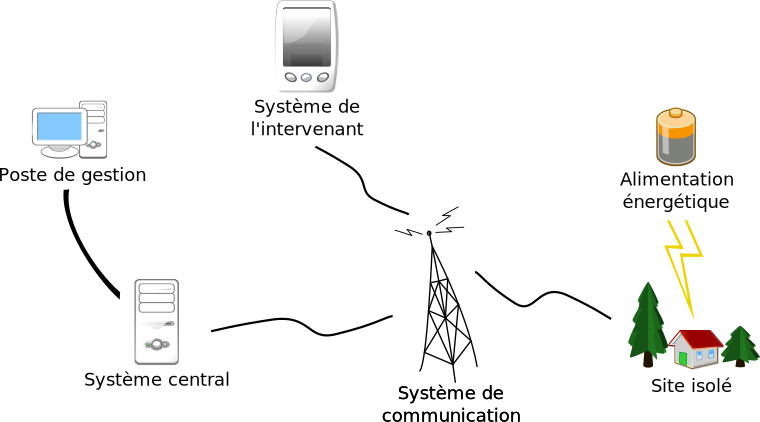
\includegraphics[width=\textwidth]{schema_architecture_generale.png}
\end {center}

\subsection{Architecture matérielle}

Détaillons maintenant l'architecture matérielle de la solution proposée :

\subsubsection{Site central}

\paragraph{Postes de travail} Il convient de mettre en place un réseau local regroupant ces postes afin d'une part de partager la connexion internet et d'autre part d'utiliser ce réseau à des fins de partage de documents.

\paragraph{Serveurs}

Tout d'abord l'hébergement et la maintenance de ces serveurs seront laissés à la charge d'un prestataire externe pour des raisons de coûts, de fiabilité, de sécurité et de haute disponibilité. Des serveurs privées seront choisis afin de garder un contrôle total du système et de garantir des performances suffisantes dans les traitements.

Dans un souci d'extensibilité et de mise à l'échelle, l'architecture serveur pourra être découpée en plusieurs serveurs chacun dédié à une fonctionnalité : serveur web, serveur applicatif, serveur hébergeant la base de données, etc. Les performances pourront être améliorées grâce à la technique du load-balancing et donc exploiter la redondance.

En cas de panne, le prestataire devra être en mesure de remettre en marche le système de manière fonctionnelle rapidement et le nombre de pannes doit être limité dans l'année (99,9\% de disponibilité préconisée, soit moins de 8,75 heures par an).

\end{document}
